% initial settings
\documentclass[12pt]{exam}
\usepackage{geometry}
\usepackage{graphicx}
\usepackage{enumitem}
\usepackage[usenames,dvipsnames]{xcolor}
\usepackage[backend=biber, style=alphabetic]{biblatex}
\usepackage{url,hyperref}

\usepackage{amsmath} % math symbols, matrices, cases, trig functions, var-greek symbols.
\usepackage{amsfonts} % mathbb, mathfrak, large sum and product symbols.
\usepackage{amssymb} % extended list of math symbols from AMS. https://ctan.math.washington.edu/tex-archive/fonts/amsfonts/doc/amssymb.pdf
\usepackage{amsthm} % theorem styling.
\usepackage{mathrsfs} % mathscr fonts.
\usepackage{yhmath} % widehat.
\usepackage{empheq} % emphasize equations, extending 'amsmath' and 'mathtools'.
\usepackage{bm} % simplified bold math. Do \bm{math-equations-here}

% geometry of paper
\geometry{
  a4paper, % 'a4paper', 'c5paper', 'letterpaper', 'legalpaper'
  asymmetric, % don't swap margins in left and right pages. as opposed to 'twoside'
  centering, % to center the content between margins
  bindingoffset=0cm,
}

% hyprlink settings
\hypersetup{
  colorlinks = true,
  linkcolor = {red!60!black},
  anchorcolor = red,
  citecolor = {green!50!black},
  urlcolor = magenta,
  }

% theorem styles
\theoremstyle{plain} % default; italic text, extra space above and below
\newtheorem{theorem}{Theorem}[section]
\newtheorem{proposition}{Proposition}[section]
\newtheorem{lemma}{Lemma}[section]
\newtheorem{corollary}{Corollary}[theorem]

\theoremstyle{definition} % upright text, extra space above and below
\newtheorem{definition}{Definition}[section]
\newtheorem{example}{Example}[section]

\theoremstyle{remark} % upright text, no extra space above or below
\newtheorem{remark}{Remark}[section]
\newtheorem*{note}{Note} %'Notes' in italics and without counter 

% renewcommands for counters
\newcommand{\propositionautorefname}{Proposition}
\newcommand{\definitionautorefname}{Definition}
\newcommand{\lemmaautorefname}{Lemma}
\newcommand{\remarkautorefname}{Remark}
\newcommand{\exampleautorefname}{Example}

\addbibresource{articles.bib}


\begin{document}

\title{MATH 6302 - Modern Algebra \\ Homework 4}

% author list
\author{
Joel Sleeba \\
}

\maketitle
\printanswers
\unframedsolutions

\begin{questions}
  
  \question
  \begin{solution}
    Let $G$ be an Abelian group with order greater than one and not isomorphic to $C_p$ for any prime $p$. Let $g \in G$ such that $g \neq e$ and $\langle g \rangle \neq G$. We claim that such an element exist. If $\langle g \rangle = G$ for all $e \neq g \in G$, then $G$ must have a prime order, which would imply $G = C_p$ for some prime $p$, contradicting our assumption. Now since $G$ is Abelian, every subgroup is normal and specifically $\langle g \rangle $ is a normal subgroup satisfying $\{ e \} \lvertneqq \langle g  \rangle \lvertneqq G$. Hence $G$ is not simple.
  \end{solution}

  \question
  \begin{solution}
    We know that arbitrary intersection of subgroups of a group is again a group. Hence we only need to check the normality of the given subgroup.
    Let $h \in \cap_{i \in I}H_i$ and $g \in G$. Since each of $H_i$ is normal $ghg^{-1} \in H_i$ for every $i \in I$. This implies $ghg^{-1} \in \cap_{i \in I}H_i$. This shows arbitrary intersection of normal subgroups is again normal.
  \end{solution}
  
  \question
  \begin{solution}
    By definition $Z(G) = \{ h \in G \ : \ gh = hg, \forall g \in G \}$. Therefore if $h \in Z(G)$ and $g, f \in G$, then $f(ghg^{-1}) = f(hgg^{-1}) = fh = hf = (gg^{-1})hf = (ghg^{-1}) f$ shows that $ghg^{-1} \in Z(G)$. Therefore $gZ(G)g^{-1} \subset Z(G)$ for all $g \in G$ and hence we see that $Z(G)$ is normal.
  \end{solution}

  \question
  \begin{solution}
    Let $r, s \in D_{14}$ be the usual rotation and flip which generate the whole group. Consider the subgroup $\langle r \rangle \leqslant D_{14}$. We claim this is a normal subgroup of $D_{14}$. Since we know that $\langle r  \rangle = \{ 1, r, r^2, r^3, r^4, r^5, r^6 \}$, to check normality, we only need to verify if $(r^as) \langle r \rangle (r^as)^{-1} \subseteq \langle r \rangle$ for $0 \le a \le 6$ (The other elements of $D_{14}$ are in $\langle  r  \rangle$ and by closure, they will satisfy $r^a \langle r  \rangle r^{-a} \subseteq \langle r  \rangle $). Now let $r^as \in D_{14}\setminus \langle r \rangle$ and $r^{b} \in \langle r \rangle $. Then since we know $r^as = sr^{-a}$ and $(r^{a}s)^{-1} = r^{a}s$, we get \begin{align*}
      (r^as) r^b (r^{ a}s)^{-1} &= (sr^{-a})r^b(r^a s) \\ 
      & = sr^{b-a+a}s \\ 
      & = sr^{b}s \\ 
      &= r^{-b}ss \\ 
      &= r^{-b} \in \langle r  \rangle 
    \end{align*}
    Hence we see that $\langle r \rangle $ is a proper nontrivial normal subgroup of $D_{14}$. 
  \end{solution}

  \question
  \begin{solution}
    $C_G(S) = \{ 1, -1 \}, N_G(S) = \{ 1, -1, j, -j \}$

    Since $ij = -ji = k$, we see that $i, j, -i, -j \notin C_G(S)$. Similarly $ki = -ik = j$ implies $ k , -k \notin C_G(S)$. Hence the only possible elements in $C_G(S)$ are $1, -1$.

    \begin{itemize}
      \item $iS = \{ -1, 1, k\} = S(-i)$ implies $i, -i \notin N_G(S)$
      \item $jS = \{ -k, k, -1 \} = S(j)$ implies $j, -j \in N_G(S)$
      \item $kS = \{ j , -j, -i \} = S(-k)$ implies $k, -k \notin N_G(S)$
    \end{itemize}
  \end{solution}

  \question
  \begin{solution}
    Let $H \trianglelefteq G$ and $\phi: G \to K$ be a surjective homomorphism. We'll show $k \phi(H) k^{-1} \subset \phi(H)$ for every $k \in K$. Let $k \in K$ and $\phi(h) \in \phi(H)$. Then since $\phi$ is surjective there exists a $g \in G$ such that $k = \phi(g)$. Hence \begin{align*}
      k \phi(h) k^{-1} & = \phi(g)\phi(h) \phi(g)^{-1} \\ 
      & = \phi(g) \phi(h) \phi(g^{-1}) \\ 
      & = \phi(ghg^{-1}) \\ 
      & = \phi(h^\prime), \quad \textrm{Since $H$ is normal $ghg^{-1} = h^\prime \in H$}
    \end{align*}
    This shows $k \phi(H) k^{-1} \subseteq \phi(H)$ for all $k \in K$. Therefore $\phi(H)$ is normal.
  \end{solution}

  \question
  \begin{solution}
    We know that if $H \trianglelefteq G$, then the canonical map $\phi: G \to G/H:= g \to gH$ is a group homomorphism. Now if $n = |g|$, then $H = \phi(e) = \phi(g^n) = \phi(g)^n = (gH)^n$ implies $n = |g|\big||gH|$. This proves our statement.
  \end{solution}

  \question
  \begin{solution}
    \begin{parts}
      \part We claim that for every rational number $0 \le r, s < 1$ where $r \neq s$, then $[r] \neq [s]$. Then by the fact that rational numbers between 0 and 1 are infinite, the result will follow.

      Let $r, s$ be rationals in $[0, 1)$ such that $[r] = [s]$. Then $r-s \in \mathbb{Z}$ which forces $r-s = 0$ since $0 \le r, s < 1$. This gives $r= s$ and our claim is proved.
      \part Let $r \mathbb{Z} \in G/H$, where $r = \frac{p}{q}$ for $p, q \in \mathbb{Z}$ with $(p, q) = 1$. Then $(r \mathbb{Z})^q = (qr) \mathbb{Z} = (q \ \frac{p}{q}) \mathbb{Z} = 0$. This shows that every element in $G/H$ has finite order.
      \part Consider $r = \frac{1}{n}$. Then $r^n = 1$. Hence $[r]^n = [r^n] = 0$. Therefore $n\big||[r]|$. Now to show $[r] = n$, we'll show that $[r]^m \neq 0$ for $1 \le m < n$. If instead $[r]^m = 0$ for some $1 \le m < n$, then $mr \in \mathbb{Z}$ by the definition. This implies $\frac{m}{n} \in \mathbb{Z}$, which is a contradiction by the assumptions on $m$. Thus we see $|[r]| = n$.
    \end{parts}
  \end{solution}

  \question
  \begin{solution}
     \begin{parts}
       \part Define $\phi: G \to K := \phi(r^ns^m) = a^nb^m$. Then $\phi(r) = a$ and $\phi(s) = b$. Now we just need to verify that this is actually a homomorphism which the following relations prove. \begin{itemize}
         \item  $\phi(r^pr^q) =  \phi(r^{p+q}) = a^{p+q} = a^pa^q = \phi(r^p)\phi(r^{q})$
         \item $\phi(r^msr^n) = \phi(r^mr^{-n}s) = \phi(r^{m-n}s) = a^{m-n}b = a^ma^{-n}b = a^mba^{n} = \phi(r^m)\phi(s)\phi(r^{n})$
         \item $\phi(r^mr^ns) = \phi(r^mr^{-n}s) = \phi(r^{m-n}s) = a^{m-n}b = a^ma^{-n}b = a^mba^{n} = \phi(r^m)\phi(s)\phi(r^{n})$
         \item $\phi(r^msr^ms) = \phi(r^mr^{-n}) = \phi(r^{m-n}) = a^{m-n} = a^ma^{-n} = a^mba^{n}b = \phi(r^m)\phi(s) \phi(r^n) \phi(s)$
       \end{itemize}
       \part Now if $\phi(r^ns^m) = a^nb^m = e$, then $a^n =e$ and $ b^m = e$. This implies $n|2$ since $|a| = 2$ and $m|2$ since $|b| = 2$. Thus we see that $r^2 \in \textrm{Ker}(\phi)$. We claim that $\textrm{Ker}(\phi) = \langle  r^2 \rangle$.

       To see this notice that $|\langle  r^2 \rangle| = 4$. If $\textrm{Ker}(\phi)$ was any bigger, then $ D_{16}/\textrm{Ker}(\phi)$ would have fewer than $16/4 = 4$ elements. But since $\phi$ is a surjective homomorphism, and $|V_4|$ has $4$ elements, this would contradict the first isomorphism theorem. Thus we see $\textrm{Ker}(\phi) = \langle r^2  \rangle$. Now by the first isomorphism theorem, we get $D_{16}/ \langle r^2  \rangle  \cong V_4$
     \end{parts}
  \end{solution}

  \question
  \begin{solution}
    Let $g, h \in G$. Since $G/Z(G) = \langle  r  \rangle $ for some $r \in G$, $g = r^mz_1$ and $g = r^nz_2$ for some $z_1, z_2 \in Z(G)$  and $m, n \in \mathbb{Z}$. Then \[
        gh = r^mz_1r^nz_2 = r^mr^nz_1z_2 = r^nr^mz_2z_1 = r^z_2r^mz_1 = hg
    \]
    Thus we see that the group is Abelian.
  \end{solution}

  \question
  \begin{solution}
    \begin{parts}
      \part We claim that the group elements $(0, 0), (1, 1), (1, 2), (2, 2), (2, 3), (2, 4), (3, 4), (3, 5)$ correspond to distinct cosets of $H$ in $G$. If $(a, b)$ is any element in $\mathbb{Z}^2$, then by adding enough $(2, 1)$ and $(2, 5)$ we can convert $(a, b)$ into one of these elements. It is clear from the below diagram that any of the orange tiles can be realigned to be at the black tile using the above transformations, which will give exactly the above representatives for distinct cosets.


      %\begin{figure}[h]
        %\centering
        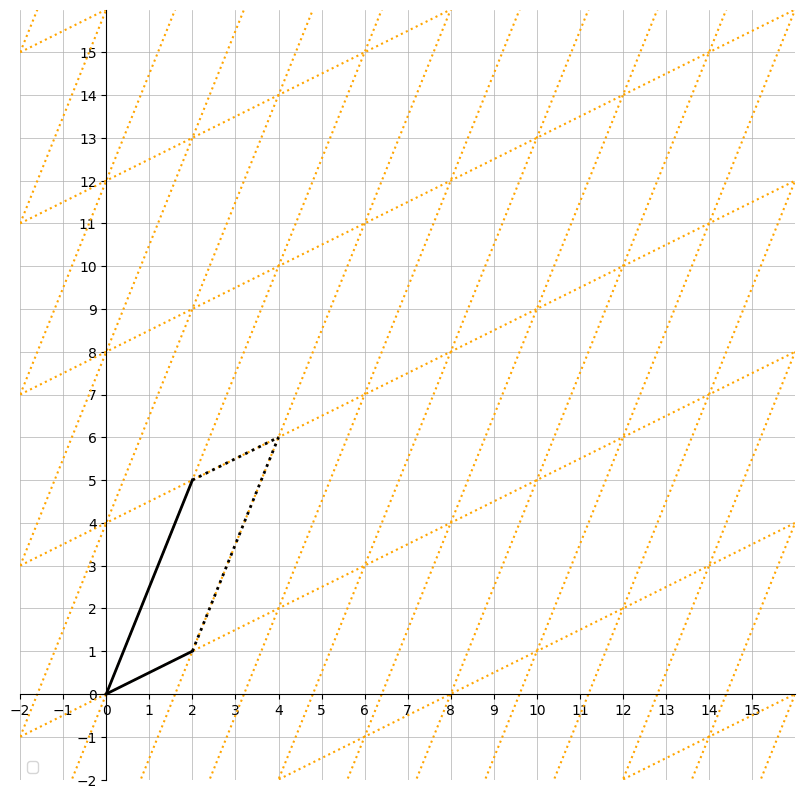
\includegraphics[width=0.8\textwidth]{assets/plot.png}
        %\caption{}
      %  \label{fig:plot}
      %\end{figure}


      \part We claim that $(1, 1)H$ generate the quotient group. To see this, \begin{itemize}
        \item $(1,1)^2 =_H (2, 2)$
        \item $(1,1)^3 =_H (3, 3) =_H (1, 2)$ by subtracting $(2, 1)$
        \item $(1, 1)^4 =_H (1, 2)+(1, 1) =_H (2, 3)$
        \item $(1,1)^5 =_H (2, 3) + (1, 1) =_H (3, 4)$
        \item $(1, 1)^6 =_H (3, 4) + (1, 1) =_H (4, 5) =_H (2, 4)$ by subtracting $(2, 1)$
        \item $(1, 1)^7 =_H (2, 4) + (1, 1) =_H (3, 5)$
        \item $(1, 1)^8 =_H (3, 5) + (1, 1) =_H (4, 6) =_H (0, 0)$ by subtracting $(2, 1)$ and $(2, 5)$.
      \end{itemize}
    \end{parts}
  \end{solution}

  \question
  \begin{solution}
    Given that $v_1, v_2$ are linearly independent vectors in $\mathbb{R}_{2}$. Then since $ \mathbb{R}_{2} $ is a vector space of dimension 2, they span $\mathbb{R}_{2}$. Hence any element in $\mathbb{R}_{2} $ can be written as the linear combination of $v_{1}$ and $v_{2} $. 
    \begin{parts}
      \part Let $H = \langle v_{1}  , v_{2}  \rangle$, $x = r_{1} v_{1} + r_{2} v_{2} \in \mathbb{R}_{2}$. Then $ x = [r_{1} ]v_{1} + [r_{2} ] v_{2} + \{r_{1} \} v_{1} + \{r_{2}\} v_{2} $ where $[x]$ is the greatest integer less than or equal to $x$ and $\{ x \}$ is the fractional part of $x$. Since $[r_{1} ] v_{1} + [r_{2} ] v_{2} \in H$, we see that $x \sim_H \{ r_{1}  \}v_{1} + \{ r_{2}  \}v_{2}$. Hence the set \[
          \{ rv_{1} + sv_{2}   \ : \  0\le r, s < 1 \}
      \]
      form a complete set of coset representatives of $H$ in $\mathbb{R}_{2}$.
      \part Let $u_{1}, u_{2} $ be any other linear independent vectors in $G = \mathbb{R}_{2}$ with $F = \langle u_{1}  , u_{2} \rangle $. Then by the similar reasoning, we get that the complete set of coset representatives for $F$ is the set \[
          \{ ru_{1} + su_{2}   \ : \  0\le r, s < 1 \}
      \]
      Moreover since $\mathbb{R}_{2} $ is Abelian and $H, F$ are subgroups, we see that $G/H, G/F$ are quotient groups.
      We claim that the map $\phi: G/H \to G/F := [rv_{1} + sv_{2}] \to [ru_{1} + su_{2}]$ is a group isomorphism. 

      To see it is well defined, let $rv_{1} + sv_{2} \sim_H pv_{1} + qv_{2}$. This is equivalent to $(r-p)v_{1} + (s-q)v_{2} \in H$ which again is equivalent to $r-p, s-q \in \mathbb{Z}$. Hence $(r-p) u_{1} + (s-q) u_{2} \in F$ and hence $ru_{1} + su_{2} \sim_F pu_{1} + qu_{2}$. Hence we see that $\phi$ is well defined.
      
      Since we know the coset representatives of $H$ and $F$ in $G$, we see that $\phi$ is surjective. Hence we only need to show that $\phi$ is an injective homomorphism. Retracing back the argument for well definess of $\phi$, we see that $\phi$ is injective. To see that $\phi$ is a homomorphism, let $[r_{1} v_{1} + r_{2} v_{2}] , [s_{1} v_{1} + s_{2} v_{2} ]\in G/H$. Then 
      \begin{align*}
        \phi([r_{1} v_{1} + r_{2} v_{2}] + [s_{1} v_{1} + s_{2} v_{2} ]) &= \phi([(r_{1}+s_{1})v_{1} + (r_{2}+s_{2})v_{2}]) \\ 
        &= [(r_{1}+s_{1})u_{1} + (r_{2}+s_{2})u_{2}] \\ 
        &= [r_{1} u_{1} + r_{2} u_{2}] + [s_{1} u_{1} + s_{2} u_{2}] 
      \end{align*}
      Hence we conclude that $\phi: G/H \to G/F$ is an isomorphism.
    \end{parts}
  \end{solution}


\end{questions}
\printbibliography[heading=bibintoc]
\end{document}
